\begin{frame}
\frametitle{Single Robot/Multi-Robot SLAM}
\begin{itemize}
\item Single Robot
\begin{itemize}
\item Very slow to map a large area
\item Increase speed $\rightarrow$ increase noise/decrease accuracy
\item Not robust: single point of failure
\end{itemize}
\item Multi-Robot SLAM (MRSLAM)
\begin{itemize}
\item SLAM with multiple robots searching the space and communicating with each other
\item May still use slower robots
\item May have robot failure, but still achieve mapping objective
%\item Two types:
%\begin{itemize}
%\item Known initial poses
%\item Encounter based
%\end{itemize}
\end{itemize}
\end{itemize}
\end{frame}

\begin{frame}
\frametitle{Challenges of MRSLAM}
\begin{itemize}
\item Often do not know initial poses
\begin{itemize}
\item Need to calculate relative poses
\end{itemize}
\item Complexity 
\begin{itemize}
\item Exploration/Coordination, efficiently move with little overlap and to get as much coverage as possible	
\end{itemize}
\item Each robot is taking measurements in its own frame
\begin{itemize}
\item How to transform the pose data?
\item How to combine the data?
\item How to create a global map?
\end{itemize} 
%\begin{itemize}
%\item 
%\end{itemize}
%\item Encounter based: robots ``observing'' each other

%\item Any portion of a feature/map can correspond, how should the individual maps be merged?
\end{itemize}
\end{frame}


\begin{frame}
\frametitle{Solving MRSLAM}
\begin{itemize}
\item Most papers solve 1 problem at a time
\begin{itemize}
\item Coordination ([Juli{\'a} et. al, 2012])
\item Map Merging ([Lazaro et. al., 2013], [Lee et. al., 2012],[Birk and Carpin, 2006], [Howard, 2006])
\end{itemize}
\item Focus: [Howard, 2006]
\begin{itemize}
\item Answers merging problem
\item All robots store sensor data for both odometry and measurements
\item Starts with a single robot, stored data integrated transformed data into the map posterior post encounter
\item Builds occupancy grid
%\item Transforms relative poses using robot encounter information to create a single map posterior

\end{itemize}

\end{itemize}
\end{frame}


\begin{frame}
\frametitle{MRSLAM Assumptions}
\begin{itemize}
\item Robots move independently of each other
\item Can determine the relative poses of each robot perfectly on an encounter
\item Continued communication post encounter
\item Robot encounters form a connected graph
\begin{center}
\begin{tabular}{cc}
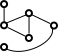
\includegraphics[width=3cm]{../FiguresAndMovies/ConnectedGraph}&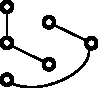
\includegraphics[width=3cm]{../FiguresAndMovies/NonConnected}\\
Connected & Not Connected
\end{tabular}
\end{center}
\end{itemize}
\end{frame}



\begin{frame}
\frametitle{[Howard, 2006] Algorithm}
\begin{itemize}
\item Occupancy Grid FastSLAM 
\item Store $(u_t,z_t,encounter_t)$ data
\item On encounter, replay past data in reverse order
\begin{center}
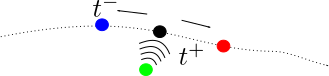
\includegraphics[height=2cm]{../FiguresAndMovies/ForwardBackward}
\end{center}
\item Post encounter integrate stored information into the map posterior in an acausal update
\item Continue communication to integrate future odometry and encounters
\end{itemize}
\end{frame}


\begin{frame}
\frametitle{Causal/Acausal Updates}
\begin{center}
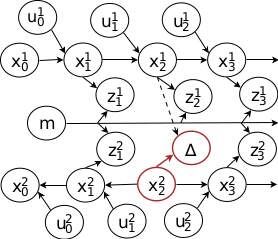
\includegraphics[height=6cm]{../FiguresAndMovies/HowardFig3}
\end{center}
\blfootnote{From [Howard, 2006]}
\end{frame}

\begin{frame}
\frametitle{[Howard, 2006] Algorithm}
\begin{itemize}
\item Robot 1 observes robot 2
\end{itemize}
\begin{center}
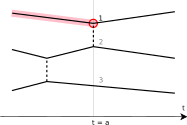
\includegraphics[height=5cm]{../FiguresAndMovies/Howard5a}
\end{center}
\blfootnote{From [Howard, 2006]}
\end{frame}


\begin{frame}
\frametitle{[Howard, 2006] Algorithm}
\begin{itemize}
\item Robot 2 observes robot 3, integrating robot 3 data
\end{itemize}
\begin{center}
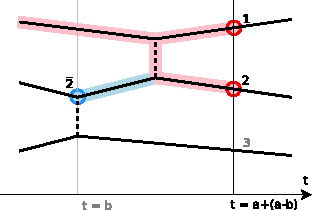
\includegraphics[height=5cm]{../FiguresAndMovies/Howard5b}
\end{center}
\blfootnote{From [Howard, 2006]}
\end{frame}

\begin{frame}
\frametitle{[Howard, 2006] Algorithm}
\begin{itemize}
\item Data is propagated, now all data is used for map
\end{itemize}
\begin{center}
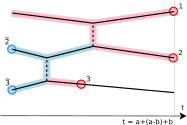
\includegraphics[height=5cm]{../FiguresAndMovies/Howard5c}
\end{center}
\blfootnote{From [Howard, 2006]}
\end{frame}

